\documentclass[twocolumn]{revtex4}

\usepackage[utf8]{inputenc}
\usepackage[T1]{fontenc}

\usepackage{textcomp}

\usepackage[ngerman]{babel}

\usepackage{amsmath}
\usepackage{amsfonts}
\usepackage{amssymb}

\usepackage{siunitx}
\sisetup{
  output-decimal-marker={,},
  separate-uncertainty
}

\usepackage{graphicx}

\usepackage{hyperref}
\hypersetup{
  colorlinks = true,
  allcolors = {black}
}



\begin{document}

\title{Atomfallen}

\author{Christopher Deutsch}

\email{christopher.deutsch@uni-bonn.de}

\affiliation{Institut, Adresse}


\begin{abstract}
%
Hier sollte eine Kurzfassung (was hat der Leser zu erwarten) von maximal 150 Worten stehen.
\\
Der ganze Fachbericht darf nicht länger als wie 2\,Seiten sein. Inklusive Referenzen. ändern sie nichts an den Seitenrändern, Zeilenabständen, ...
%
\end{abstract}

\maketitle

\section{Einleitung}
1/2 Spalte...

\section{Hauptteil}
3-4 Bilder gesamter Fachbericht


Vermeiden Sie ungünstige Zeilenumbrüche zwischen Beschreibung und Variablen -- ...~ die Strecke~$s$ ... --  mit~\verb"~" eintippen um einen Zeilenumbruch zu verhindern. Sieht dann so aus: \verb"die Strecke~$s$".

Auf alle Abbildungen im Text verweisen. Reihenfolge einhalten (erst Abb.~1, dann Abb.~2 ... und zwar  so: ... Abb.\,\ref{fig:Bild} ... und so gehört es eingetippt: \verb"Abb.\,\ref{fig:Bild}"


\begin{figure}[bbb]
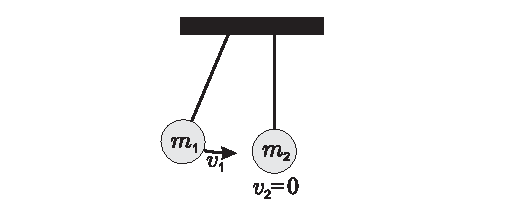
\includegraphics{Bild}
%
\caption{\label{fig:Bild}
%
Die Bildunterschrift muss voll erklärend sein: Variablen im Bild müssen in der Bildunterschrift erläutert werden. Zwei Massen $m_1$ und $m_2$ ... DAs führt zu Wiederholungen im Text, und das ist ok!
%
}
%
\end{figure}


Abbildungen wenn möglich als Graustufenbild erstellen. Maximale Breite ist 80\,mm. Sonst muss man ein Bild über zwei Spalten einfügen (auch ok). 
Auch in den Abbildungen selber auf die Schriftgrösse achten: nicht beliebig viel größer als wie im Text, und aber auch nicht substantiell kleiner.


\begin{thebibliography}{}

\bibitem{Alexe}
M.\,Alexe and A.\,Gruverman, eds., {\it Nanoscale Characterisation of
Ferroelectric Materials} (Springer, Berlin; New York, 2004) 1st ed.

\end{thebibliography}


\end{document}
